\documentclass[12pt,t]{beamer}
% xcolor and define colors -------------------------
\usepackage{xcolor}

% https://www.viget.com/articles/color-contrast/
\definecolor{purple}{HTML}{695693}
\definecolor{navy}{HTML}{567293}
\definecolor{ruby}{HTML}{9a2515}
\definecolor{alice}{HTML}{107895}
\definecolor{daisy}{HTML}{EBC944}
\definecolor{coral}{HTML}{F26D21}
\definecolor{kelly}{HTML}{829356}
\definecolor{cranberry}{HTML}{E64173}
\definecolor{jet}{HTML}{131516}
\definecolor{asher}{HTML}{555F61}
\definecolor{slate}{HTML}{314F4F}

% Main theme colors
\definecolor{accent}{HTML}{107895}
\definecolor{accent2}{HTML}{9a2515}

\newcommand\navy[1]{{\color{navy}#1}}
\newcommand\purple[1]{{\color{purple}#1}}
\newcommand\kelly[1]{{\color{kelly}#1}}
\newcommand\ruby[1]{{\color{ruby}#1}}
\newcommand\alice[1]{{\color{alice}#1}}
\newcommand\daisy[1]{{\color{daisy}#1}}
\newcommand\coral[1]{{\color{coral}#1}}
\newcommand\cranberry[1]{{\color{cranberry}#1}}
\newcommand\slate[1]{{\color{slate}#1}}
\newcommand\jet[1]{{\color{jet}#1}}
\newcommand\asher[1]{{\color{asher}#1}}

\newcommand\bgNavy[1]{{\colorbox{navy!80!white}{\textcolor{white}{#1}}}}
\newcommand\bgPurple[1]{{\colorbox{purple!80!white}{\textcolor{white}{#1}}}}
\newcommand\bgKelly[1]{{\colorbox{kelly!80!white}{\textcolor{white}{#1}}}}
\newcommand\bgRuby[1]{{\colorbox{ruby!80!white}{\textcolor{white}{#1}}}}
\newcommand\bgAlice[1]{{\colorbox{alice!80!white}{\textcolor{white}{#1}}}}
\newcommand\bgDaisy[1]{{\colorbox{daisy!80!white}{\textcolor{white}{#1}}}}
\newcommand\bgCoral[1]{{\colorbox{coral!80!white}{\textcolor{white}{#1}}}}
\newcommand\bgCranberry[1]{{\colorbox{cranberry!80!white}{\textcolor{white}{#1}}}}


% Beamer Options -------------------------------------

% Background
\setbeamercolor{background canvas}{bg = white}

% Change text margins
\setbeamersize{text margin left = 15pt, text margin right = 15pt} 

% \alert
\setbeamercolor{alerted text}{fg = accent2}

% Frame title
\setbeamercolor{frametitle}{bg = white, fg = jet}
\setbeamercolor{framesubtitle}{bg = white, fg = accent}
\setbeamerfont{framesubtitle}{size = \small, shape = \itshape}

% Block
\setbeamercolor{block title}{fg = white, bg = accent2}
\setbeamercolor{block body}{fg = jet, bg = jet!10!white}

% Title page
\setbeamercolor{title}{fg = jet}
\setbeamercolor{subtitle}{fg = accent}

%% Custom \maketitle and \titlepage
\setbeamertemplate{title page}
{
    %\begin{centering}
        \vspace{20mm}
        {\Large \usebeamerfont{title}\usebeamercolor[fg]{title}\inserttitle}\\ \vskip0.25em%
        \ifx\insertsubtitle\@empty%
        \else%
          {\usebeamerfont{subtitle}\usebeamercolor[fg]{subtitle}\insertsubtitle\par}%
        \fi% 
        {\vspace{10mm}\insertauthor}\\
        {\color{asher}\small{\insertdate}}\\
    %\end{centering}
}

% Table of Contents
\setbeamercolor{section in toc}{fg = accent!70!jet}
\setbeamercolor{subsection in toc}{fg = jet}

% Button 
\setbeamercolor{button}{bg = accent}

% Remove navigation symbols
\setbeamertemplate{navigation symbols}{}

% Optional: page numbers at bottom
\addtobeamertemplate{navigation symbols}{}{%
    \usebeamerfont{footline}%
    \hspace{1em}%
    \alice{\insertframenumber/\inserttotalframenumber}
    \vspace*{1.5mm}
}


% Table and Figure captions
\setbeamercolor{caption}{fg=jet!70!white}
\setbeamercolor{caption name}{fg=jet}
\setbeamerfont{caption name}{shape = \itshape}

% Bullet points

%% Fix left-margins
\settowidth{\leftmargini}{\usebeamertemplate{itemize item}}
\addtolength{\leftmargini}{\labelsep}

%% enumerate item color
\setbeamercolor{enumerate item}{fg = accent}
\setbeamerfont{enumerate item}{size = \small}
\setbeamertemplate{enumerate item}{\insertenumlabel.}

%% enumerate subitem color
\setbeamercolor{enumerate subitem}{fg = accent!60!white}
\setbeamerfont{enumerate subitem}{size = \small}
\setbeamertemplate{enumerate subitem}{\insertenumlabel.}

%% itemize
\setbeamercolor{itemize item}{fg = accent!70!white}
\setbeamerfont{itemize item}{size = \small}
\setbeamertemplate{itemize item}[circle]

%% right arrow for subitems
\setbeamercolor{itemize subitem}{fg = accent!60!white}
\setbeamerfont{itemize subitem}{size = \small}
\setbeamertemplate{itemize subitem}{$\rightarrow$}

\setbeamertemplate{itemize subsubitem}[square]
\setbeamercolor{itemize subsubitem}{fg = jet}
\setbeamerfont{itemize subsubitem}{size = \small}

% References

%% Bibliography Font, roughly matching aea
\setbeamerfont{bibliography item}{size = \footnotesize}
\setbeamerfont{bibliography entry author}{size = \footnotesize, series = \bfseries}
\setbeamerfont{bibliography entry title}{size = \footnotesize}
\setbeamerfont{bibliography entry location}{size = \footnotesize, shape = \itshape}
\setbeamerfont{bibliography entry note}{size = \footnotesize}

\setbeamercolor{bibliography item}{fg = jet}
\setbeamercolor{bibliography entry author}{fg = accent!60!jet}
\setbeamercolor{bibliography entry title}{fg = jet}
\setbeamercolor{bibliography entry location}{fg = jet}
\setbeamercolor{bibliography entry note}{fg = jet}

%% Remove bibliography symbol in slides
\setbeamertemplate{bibliography item}{}





% Links ----------------------------------------------

\usepackage{hyperref}
\hypersetup{
  colorlinks = true,
  linkcolor = accent2,
  filecolor = accent2,
  urlcolor = accent2,
  citecolor = accent2,
}


% Line spacing --------------------------------------
\usepackage{setspace}
% \setdisplayskipstretch{2}
\setstretch{1.3}


% \begin{columns} -----------------------------------
\usepackage{multicol}


% Fonts ---------------------------------------------
% Beamer Option to use custom fonts
\usefonttheme{professionalfonts}

% \usepackage[utopia, smallerops, varg]{newtxmath}
% \usepackage{utopia}
\usepackage[sfdefault,light]{roboto}

% Small adjustments to text kerning
\usepackage{microtype}



% Remove annoying over-full box warnings -----------
\vfuzz2pt 
\hfuzz2pt


% Table of Contents with Sections
\setbeamerfont{myTOC}{series=\bfseries, size=\Large}
\AtBeginSection[]{
        \frame{
            \frametitle{Roadmap}
            \tableofcontents[current]   
        }
    }


% References ----------------------------------------
\usepackage[
    citestyle= authoryear,
    style = authoryear,
    natbib = true, 
    backend = biber
]{biblatex}

% Smaller font-size for references
\renewcommand*{\bibfont}{\small}

% Remove "In:"
\renewbibmacro{in:}{}

% Color citations for slides
\newenvironment{citecolor}
    {\footnotesize\begin{color}{accent2}}
    {\end{color}}

\newcommand{\citetcolor}[1]{{\footnotesize\textcolor{gray}{\citet{#1}}}}
\newcommand{\citepcolor}[1]{{\footnotesize\textcolor{gray}{\citep{#1}}}}

% Tables -------------------------------------------
% Tables too big
% \begin{adjustbox}{width = 1.2\textwidth, center}
\usepackage{adjustbox}
\usepackage{array}
\usepackage{threeparttable, booktabs, adjustbox}
    
% Fix \input with tables
% \input fails when \\ is at end of external .tex file

\makeatletter
\let\input\@@input
\makeatother

% Tables too narrow
% \begin{tabularx}{\linewidth}{cols}
% col-types: X - center, L - left, R -right
% Relative scale: >{\hsize=.8\hsize}X/L/R
\usepackage{tabularx}
\newcolumntype{L}{>{\raggedright\arraybackslash}X}
\newcolumntype{R}{>{\raggedleft\arraybackslash}X}
\newcolumntype{C}{>{\centering\arraybackslash}X}

% Figures

% \imageframe{img_name} -----------------------------
% from https://github.com/mattjetwell/cousteau
\newcommand{\imageframe}[1]{%
    \begin{frame}[plain]
        \begin{tikzpicture}[remember picture, overlay]
            \node[at = (current page.center), xshift = 0cm] (cover) {%
                \includegraphics[keepaspectratio, width=\paperwidth, height=\paperheight]{#1}
            };
        \end{tikzpicture}
    \end{frame}%
}

% subfigures
\usepackage{subfigure}

% Strikeout text
\usepackage{cancel}

% Highlight slide -----------------------------------
% \begin{transitionframe} Text \end{transitionframe}
% from paulgp's beamer tips
\newenvironment{transitionframe}{
    \setbeamercolor{background canvas}{bg=accent!60!black}
    \begin{frame}\color{accent!10!white}\LARGE\centering
}{
    \end{frame}
}


% Table Highlighting --------------------------------
% Create top-left and bottom-right markets in tabular cells with a unique matching id and these commands will outline those cells
\usepackage[beamer,customcolors]{hf-tikz}
\usetikzlibrary{calc,fit,shapes.misc,backgrounds}
\usepackage{pgfplots}
\pgfplotsset{compat = newest}
\usetikzlibrary{positioning, arrows.meta}
\usepgfplotslibrary{fillbetween}

% halo around text
%https://tex.stackexchange.com/questions/18472/tikz-halo-around-text
\usepackage[outline]{contour} 
\contourlength{1.2pt}
\tikzset{
  contour text/.style={node contents={\contour{white}{#1}}},
  halo text node/.style={circle, draw, pattern=north east lines}
}


\def\arraystretch{0.75}

% To set the hypothesis highlighting boxes red.
\newcommand\marktopleft[1]{%
    \tikz[overlay,remember picture] 
        \node (marker-#1-a) at (0,1.5ex) {};%
}
\newcommand\markbottomright[1]{%
    \tikz[overlay,remember picture] 
        \node (marker-#1-b) at (0,0) {};%
    \tikz[accent!80!jet, ultra thick, overlay, remember picture, inner sep=4pt]
        \node[draw, rectangle, fit=(marker-#1-a.center) (marker-#1-b.center)] {};%
}


\author{Michael R. Karas}
\title{Lecture 3 - Consumer Preferences and Utility}
\subtitle{ECON 3070 - Intermediate Microeconomic Theory}
\date{January X, 2025}

\begin{document}

% ------------------------------------------------------------------------------------------------
\begin{frame}
  \titlepage
\end{frame}
% ------------------------------------------------------------------------------------------------

% ------------------------------------------------------------------------------------------------
\begin{frame}{Overview}
  In this lecture, we will consider the following:
  \begin{enumerate}
    \item How we can represent and analyze consumer preferences.
    \item Basic assumptions about consumer preferences.
    \item Utility functions  - Functions representing an individual's preferences for one or more goods.
    \item Indifference curves as a graphical representation of consumer preferences.
    \item What happens to consumers' desire for a good as they consume more of it?
  \end{enumerate}
\end{frame}
% ------------------------------------------------------------------------------------------------


% ------------------------------------------------------------------------------------------------
\begin{frame}{Consumer Preferences}
  We all face trade-offs when it comes to our budget. Most people can't afford to buy everything they want.

  \begin{itemize}
    \item So how do we choose?

    \item Need a way of deciding between two or more `baskets' of items.
  \end{itemize}
\end{frame}
% ------------------------------------------------------------------------------------------------

% ------------------------------------------------------------------------------------------------
\begin{frame}{Consumer Preferences}
  \textbf{Consumer preferences} tell us how an individual would rank any two baskets of goods (not considering their cost). We make a few assumptions about consumer preferences:

  \bigskip
  \begin{itemize}
    \item Completeness: Consumer is able to rank any two baskets.
    \item Transitivity: If basket A is preferred to basket B, and B is preferred to C, then A is preferred to C.
    \item More is Better: Having more of a good is better for the consumer.
  \end{itemize}
\end{frame}
% ------------------------------------------------------------------------------------------------

% ------------------------------------------------------------------------------------------------
\begin{frame}{Consumer Preferences}
  \textbf{Ordinal rankings} give us information about the \textit{order} in which a consumer ranks baskets. \emph{e.g. 1st, 2nd, 3rd, ...}


  \pause\bigskip
  \textbf{Cardinal rankings} give us information about the intensity of consumer preferences. \emph{I like this one 10, I like this one 25, etc.}

  \begin{itemize}
    \item What do these numbers mean? Units?
  \end{itemize}
\end{frame}
% ------------------------------------------------------------------------------------------------

% ------------------------------------------------------------------------------------------------
\begin{frame}{Utility Functions}
  \textbf{Utility} refers to consumer happiness or wellbeing. If a consumer prefers one basket to another, that basket is said to provide greater \textit{utility}.
  
  \pause\bigskip
  \textbf{Utility functions} measure the level of satisfaction that a consumer receives from any basket of goods. Examples:
  \begin{itemize}
    \item $U(X,Y) = 3X + 4Y$
    \item $U(X,Y) = X^{\frac{1}{2}}Y^{\frac{1}{2}}$
    \item $U(X,Y) = \log(XY)$
  \end{itemize}
\end{frame}
% ------------------------------------------------------------------------------------------------

% ------------------------------------------------------------------------------------------------
\begin{frame}{Why are we using functions?}
  Utility cannot actually be measured, so the exact specification is arbitrary.

  \begin{itemize}
    \item What matters is not the level of utility derived from a basket.
    
    \item It is how that level of utility \textit{compares} to other baskets. 
  \end{itemize}

  \pause\bigskip 
  Utility explains how a person think about \bgNavy{trade-offs}

  \pause\bigskip 
  Utility cannot be compared \textit{between} individuals, only \textit{within} an individual. 

\end{frame}
% ------------------------------------------------------------------------------------------------

% ------------------------------------------------------------------------------------------------
\begin{frame}{\navy{Trade-offs} and `Marginal Utility'}
  \textbf{Marginal utility} refers to the rate at which total utility changes as the level of consumption of one good rises (holding constant the level of consumption of all other goods), and is given by:

  $$ 
    MU_x = \frac{\Delta U}{\Delta	x}
  $$ 
  
  We will see that marginal utility is very helpful since it lets us compare \emph{on the margin} how people compare more of different goods.

  \pause 
  \begin{itemize}
    \item This is also the formula for the slope of the utility function. ($U$ on the $y$-axis, good $x$ on the $x$-axis)
    \item It is also the partial derivative with respect to $x$: $\frac{\delta U(x)}{\delta x}$.
  \end{itemize}
\end{frame}
% ------------------------------------------------------------------------------------------------

% ------------------------------------------------------------------------------------------------
\begin{frame}[c]{Diminishing Returns}
  \begin{center}
    Why do you stop eating pizza when you do?
  \end{center}
\end{frame}
% ------------------------------------------------------------------------------------------------

% ------------------------------------------------------------------------------------------------
\begin{frame}{Marginal Utility}
  \textbf{Diminishing marginal utility} means that as an individual consumes more of a good, their additional (or marginal) utility from that good decreases.

  \begin{itemize}
    \item Think about the additional satisfaction you get from eating more pizza...

    \item Or watching additional episodes of a tv show on Netflix.

    \pause
    \item At some point, we might have negative marginal utility, but for amounts that the consumer is likely to purchase, this probably is true.
  \end{itemize}
\end{frame}
% ------------------------------------------------------------------------------------------------

% ------------------------------------------------------------------------------------------------
\begin{frame}
  \bgCranberry{Try It Yourself}

  \bigskip
  Suppose that a consumer's preference can be represented by the utility function $U(X,Y) = 4X^\frac{1}{2} Y^\frac{1}{2}$. 
  
  What is the consumer's marginal utility function for good $X$?
\end{frame}
% ------------------------------------------------------------------------------------------------

% ------------------------------------------------------------------------------------------------
\begin{frame}{\navy{Tradeoffs} and Indifference Curves}
  In the case where a consumer is choosing quantities of two goods, the consumer's utility function can be represented graphically using indifference curves.

  \begin{itemize}
    \item In the case where a consumer is choosing quantities of two goods, the consumer's utility function can be represented graphically using indifference curves.

    \item An \textbf{indifference curve} represents bundles of two goods which provide a consumer with the same level of utility.

    \item Consider the following illustration of a utility function with two goods: 
  \end{itemize}
\end{frame}
% ------------------------------------------------------------------------------------------------

% ------------------------------------------------------------------------------------------------
\begin{frame}
  \vspace{-5mm}
  \begin{figure}
    \caption{Indifference Curves in 2D}
    
    \begin{tikzpicture}
      \begin{axis}[
        width = 10cm,
        height = 8cm,
        xmin = 0, xmax = 12,
        ymin = 0, ymax = 12,
        axis lines = left,
        xtick = {2, 4, 6, 8, 10}, 
        ytick = {2, 4, 6, 8, 10},
        x label style={at={(axis description cs:0.5,-0.07)},anchor=north},
        y label style={at={(axis description cs:-0.07,.5)},anchor=south},
        xlabel = {\small $x$, units of food},
        ylabel = {\small $y$, units of clothing},
        clip = false,
      ]
        % Indifference curve
        \addplot[domain = 0:12, restrict y to domain = 0:12, samples = 400, color = alice!25!white, thick]{4/x};
        \node [right,color=alice!25!white] at (axis cs: 12, 4/12) {$U = 2$};
        
        \addplot[domain = 0:12, restrict y to domain = 0:12, samples = 400, color = alice!50!white, thick]{16/x};
        \node [right,color=alice!50!white] at (axis cs: 12, 16/12) {$U = 4$};

        \addplot[domain = 0:12, restrict y to domain = 0:12, samples = 400, color = alice!75!white, thick]{36/x};
        \node [right,color=alice!75!white] at (axis cs: 12, 3) {$U = 6$};
        % the published did this wrong, but I'm keeping it to match the last figure
        
        \addplot[domain = 0:12, restrict y to domain = 0:12, samples = 400, color = alice!100!white, thick]{64/x};
        \node [right,color=alice!100!white] at (axis cs: 12, 64/12) {$U = 8$}; 
        % the published did this wrong, but I'm keeping it to match the last figure

        % Labels
        \node [anchor = north east] at (current axis.right of origin) {$x$};
        \node [above] at (current axis.above origin) {$y$};

        % Highlight Indifference Curve
        \addplot[color = black, mark = *, only marks, mark size = 2pt] 
        coordinates {(2,8) (4,4) (8,2)};

        \addplot[color = black, dotted, thick] 
          coordinates {(0, 8) (2, 8) (2, 0)};
        \node [anchor = south west] at (axis cs:2, 8) {$A$};

        \addplot[color = black, dotted, thick] 
          coordinates {(0, 4) (4, 4) (4, 0)};
        \node [anchor = south west] at (axis cs:4, 4) {$B$};

        \addplot[color = black, dotted, thick] 
          coordinates {(0, 2) (8, 2) (8, 0)};
        \node [anchor = south west] at (axis cs:8, 2) {$C$};


      \end{axis}
    \end{tikzpicture}
  \end{figure}
\end{frame}

% ------------------------------------------------------------------------------------------------

% ------------------------------------------------------------------------------------------------
\begin{frame}
  \begin{figure}
    \caption{Indifference Curves}
    
    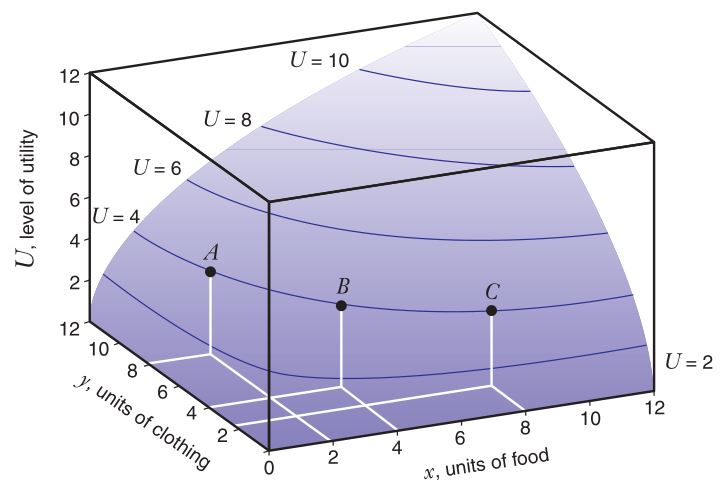
\includegraphics[width= 0.8\linewidth]{figures/fig3_4.jpg}
  \end{figure}
\end{frame}
% ------------------------------------------------------------------------------------------------

% ------------------------------------------------------------------------------------------------
\begin{frame}{How do you draw an indifference curve?}
  Say the utility function is $U(x, y) = x + 2y$. To draw an indifference curve:

  \bigskip
  \begin{enumerate}
    \item Pick a value of utility $\bar{U}$. Solve for $y$.
    
    \emph{e.g.} $\bar{U} = 2 = x + 2y \implies y = 1 - \frac{1}{2x}$

    \item Pick points and `trace out' indifference curve shape. 
    
    In this case, we have a line, so drawing it should be easy.
  \end{enumerate}

  \bigskip
  \begin{center}
    \emph{Tip: Pick a $\bar{U}$ so the math works well.}
  \end{center}
\end{frame}
% ------------------------------------------------------------------------------------------------

% ------------------------------------------------------------------------------------------------
\begin{frame}
  \bgCranberry{Try It Yourself}

  \bigskip
  Draw three indifference curves for the utility function $U(x, y) = 2x + 2y$
\end{frame}
% ------------------------------------------------------------------------------------------------

% ------------------------------------------------------------------------------------------------
\begin{frame}{Properties of Indifference Curves}
  Indifference curves have four properties:

  \begin{itemize}
    \item If both products are 'goods', curves slope downward.

    \item Indifference curves \textbf{cannot} intersect.

    \item Every consumption basket lies on only one indifference curve.

    \item Indifference curves are not "thick".
  \end{itemize}

\end{frame}
% ------------------------------------------------------------------------------------------------

% ------------------------------------------------------------------------------------------------
\begin{frame}{Marginal Rate of Substitution}
  Note that for a consumer to stay on a given indifference curve (keeping utility constant), if they receive more of one good, they must give up a certain amount of the other. \navy{Why is that?}
  
  \pause\bigskip
  \begin{itemize}
    \item Just increase one good $\implies$ higher utility
    \item Just decrease one good $\implies$ lower utility
    \item Need to increase one and decrease another to keep utility constant
  \end{itemize}

  \pause\bigskip
  But how much of the other good do we have to give up to stay on the indifference curve?
\end{frame}
% ------------------------------------------------------------------------------------------------

% ------------------------------------------------------------------------------------------------
\begin{frame}{Marginal Rate of Substitution}
  But how much of the other good do we have to give up to stay on the indifference curve? This is the \textbf{marginal rate of substitution (MRS)}

  \begin{itemize}
    \item The rate at which a consumer must substitute one good for another to stay on the same indifference curve is given by $\Delta y / \Delta x$.

    \item $MRS_{x,y}$ is therefore also the slope of the indifference curves ($\Delta y / \Delta x$)
  \end{itemize}

\end{frame}
% ------------------------------------------------------------------------------------------------

% ------------------------------------------------------------------------------------------------
\begin{frame}
  \vspace{-5mm}
  \begin{figure}
    \caption{Marginal Rate of Substitution}
    
    \begin{tikzpicture}
      \begin{axis}[
        width = 10cm,
        height = 8cm,
        xmin = 0, xmax = 12,
        ymin = 0, ymax = 12,
        axis lines = left,
        xtick = {2, 4, 6, 8, 10}, 
        ytick = {2, 4, 6, 8, 10},
        x label style={at={(axis description cs:0.5,-0.07)},anchor=north},
        y label style={at={(axis description cs:-0.07,.5)},anchor=south},
        xlabel = {\small $x$, hamburgers per week},
        ylabel = {\small $y$, glasses of lemonader per week},
        clip = false,
      ]

        
        \addplot[domain = 0:12, restrict y to domain = 0:12, samples = 400, color = alice!50!white, thick]{16/x};
        \node [right,color=alice!50!white] at (axis cs: 12, 16/12) {$U = 4$};

        % Highlight Indifference Curve
        \addplot[color = black, mark = *, only marks, mark size = 2pt] 
        coordinates {(2,8) (4,4) (5, 3.2) (8,2)};
        
        % MRS = y/x
        \node [anchor = south west] at (axis cs:2, 8) {$A$};
        \addplot[color = black, thick] 
          coordinates {(1.6, 9.4) (2, 8) (2.4, 6.4)};

        \node [anchor = south west] at (axis cs:4, 4) {$B$};
        \addplot[color = black, thick] 
          coordinates {(2.8, 5.2) (4, 4) (5.2, 2.8)};

        \node [anchor = south west] at (axis cs:5, 3.2) {$C$};
        \addplot[color = black, thick] 
          coordinates {(3.8, 3.968) (5, 3.2) (6.2, 2.432)};

        \node [anchor = south west] at (axis cs:8, 2) {$D$};
        \addplot[color = black, thick] 
          coordinates {(6.8, 2.3) (8, 2) (9.2, 1.7)};


      \end{axis}
    \end{tikzpicture}
  \end{figure}
\end{frame}
% ------------------------------------------------------------------------------------------------

% ------------------------------------------------------------------------------------------------
\begin{frame}
  \bgCranberry{Try It Yourself}

  \bigskip
  Suppose that Tom is indifferent between two meals: Meal A contains 3 cheeseburgers (C), and 1 large french fry (F). Meal B contains 2 cheeseburgers and 3 large french fries. What is Tom's $MRS_{C,F}$?

  \emph{Remember: $MRS_{C,F} = \vert \frac{\Delta F}{\Delta C} \vert$}
\end{frame}
% ------------------------------------------------------------------------------------------------

% ------------------------------------------------------------------------------------------------
\begin{frame}{MRS and Marginal Utility}
  Can also express MRS as ratio of marginal utilities of two goods
  \begin{itemize}
    \item To stay on the same indifference curve, for any small change in quantity of good $x$, \textbf{the change in utility from good $y$ must offset the change in utility from good $x$.}
    
    That is, 
    $$
      MU_x * \Delta x = - MU_y * \Delta y
    $$ 
  \end{itemize}
  
  \pause\bigskip
  Rearranging the terms, gives us our formula we will use for the class 
  $$
    -\frac{\Delta y}{\Delta x} = \frac{MU_x}{MU_y} = MRS_{x,y}
  $$
\end{frame}
% ------------------------------------------------------------------------------------------------

% ------------------------------------------------------------------------------------------------
\begin{frame}{How to interpret MRS}
  The way you interpret MRS is: 
  
  \bigskip
  For a $1$ unit decrease of $x$, you would have to get $MRS_{x,y}$ units of $y$ (and vice-versa)
  

  \pause\bigskip
  $MRS_{x,y}$ means you \textbf{substitute $x$ for $y$}
\end{frame}
% ------------------------------------------------------------------------------------------------

% ------------------------------------------------------------------------------------------------
\begin{frame}
  \bgCranberry{Try It Yourself}

  \bigskip
  Calculate the marginal rate of substitution, $MRS_{x,y}$, for the following utility functions:
  $$
    U(x,y) = 2x + y \quad\text{ and }\quad U(x,y) = x^{\frac{1}{2}} y^{\frac{1}{2}};
  $$
\end{frame}
% ------------------------------------------------------------------------------------------------

% ------------------------------------------------------------------------------------------------
\begin{frame}{Diminishing Marginal Rate of Substitution}
  Remember that for many goods, as consumption increases, the additional utility gained from consuming the good (MU) decreases.

  $$
    MRS_{x,y} = \frac{MU_x}{MU_{y}}
  $$
  
  \begin{itemize}
    \item More of good $y$ $\implies$ lower $MU_{y}$ $\implies$ higher $MRS_{x,y}$. 
    
    \pause
    \item Therefore to get one unit of good $x$, the more good $y$ we would give up for . 

    \item Said another way, we would be willing to give less of good $x$ for each additional unit of good $y$ we consume, holding $x$ constant.
  \end{itemize}
\end{frame}
% ------------------------------------------------------------------------------------------------

% ------------------------------------------------------------------------------------------------
\begin{frame}{The three utility functions in this class}
  There are three kinds of utility functions we will give you in this course. 
  
  \bigskip\bigskip
  If you want to do well in this class, you should practice these three functions a bunch \emph{(calculate MRS, draw indifference curves, and later on calculate demand curves for $x$ and $y$)}
\end{frame}
% ------------------------------------------------------------------------------------------------

% ------------------------------------------------------------------------------------------------
\begin{frame}{Preference \#1: Perfect Substitutes}
  If two goods are \textbf{perfect substitutes} for a consumer, then the marginal rate of substitution is constant (would always trade them at a constant rate)

  \bigskip
  These are given by $U(x,y) = ax + by$ where $a$ and $b$ are two numbers that describe the rate you would trade them.
\end{frame}
% ------------------------------------------------------------------------------------------------

% ------------------------------------------------------------------------------------------------
\begin{frame}{Preference \#1: Perfect Substitutes}
  \bgCranberry{Try It Yourself}

  \bigskip
  Calculate the $MRS_{x,y}$ for $U(x,y) = ax + by$. Then draw two indifference curves
\end{frame}
% ------------------------------------------------------------------------------------------------

% ------------------------------------------------------------------------------------------------
\begin{frame}
  \vspace{-5mm}
  \begin{figure}
    \caption{Perfect Substitutes}
    
    \begin{tikzpicture}
      \begin{axis}[
        width = 10cm,
        height = 8cm,
        xmin = 0, xmax = 9,
        ymin = 0, ymax = 5,
        axis lines = left,
        xtick = {4, 8}, 
        ytick = {2, 4},
        x label style={at={(axis description cs:0.5,-0.07)},anchor=north},
        y label style={at={(axis description cs:-0.07,.5)},anchor=south},
        xlabel = {\small $x$, iPhones},
        ylabel = {\small $y$, Phone Cases},
        clip = false,
      ]
        % Indifference curve
        \addplot[domain = 0:4, samples = 400, color = alice!50!white, thick]{2 - x/2};
        \node [right,color=alice!50!white] at (axis cs: 3, 1) {$U = 4$};
        
        \addplot[domain = 0:8, samples = 400, color = alice!100!white, thick]{4 - x/2};
        \node [right,color=alice!100!white] at (axis cs: 4, 2.5) {$U = 8$};
      \end{axis}
    \end{tikzpicture}
  \end{figure}
\end{frame}
% ------------------------------------------------------------------------------------------------

% ------------------------------------------------------------------------------------------------
\begin{frame}{Preferences \#2: Cobb-Douglas}
  Utility functions of the form $U=x^\alpha  y^\beta$ are known as \textbf{Cobb-Douglas Utility Functions}. $\alpha$ and $\beta$ are numbers (typically between $0$ and $1$)

  \bigskip
  Note this utitlity function displays diminishing marginal rates of substitutions which is the most common case in the real world.
\end{frame}
% ------------------------------------------------------------------------------------------------

% ------------------------------------------------------------------------------------------------
\begin{frame}{Preference \#2: Cobb-Douglas}
  \bgCranberry{Try It Yourself}

  \bigskip
  Calculate the $MRS_{x,y}$ for $U(x,y) = x^{\frac{1}{3}} y^{\frac{2}{3}}$. Then draw two indifference curves
\end{frame}
% ------------------------------------------------------------------------------------------------

% ------------------------------------------------------------------------------------------------
\begin{frame}
  \vspace{-5mm}
  \begin{figure}
    \caption{Cobb-Douglas}
    
    \begin{tikzpicture}
      \begin{axis}[
        width = 10cm,
        height = 8cm,
        xmin = 0, xmax = 12,
        ymin = 0, ymax = 12,
        axis lines = left,
        xtick = {2, 4, 6, 8, 10},
        ytick = {2, 4, 6, 8, 10},
        x label style={at={(axis description cs:0.5,-0.07)},anchor=north},
        y label style={at={(axis description cs:-0.07,.5)},anchor=south},
        xlabel = {\small $P$, pancakes},
        ylabel = {\small $W$, waffles},
        clip = false,
      ]
        % Indifference curve
        \addplot[domain = 0:10, restrict y to domain = 0:10, samples = 400, color = alice!50!white, thick]{4/x};
        \node [right,color=alice!50!white] at (axis cs: 2.25, 2.25) {$U = 2$};
        
        \addplot[domain = 0:10, restrict y to domain = 0:10, samples = 400, color = alice!100!white, thick]{16/x};
        \node [right,color=alice!100!white] at (axis cs: 4.25, 4.25) {$U = 4$};
      \end{axis}
    \end{tikzpicture}
  \end{figure}
\end{frame}
% ------------------------------------------------------------------------------------------------

% ------------------------------------------------------------------------------------------------
\begin{frame}{Preference \#3: Perfect Complements}
  If two goods are \textbf{perfect complements} for a consumer, then the consumer only consumes the good in a constant proportion.

  \bigskip
  They are given by $U(x,y) = \min\big(ax, by\big)$. You will always consumer such that $ax = by$. Why?

  \pause\bigskip
  Holding $y$ fixed:

  \begin{itemize}
    \item if $ax < by$, then you are spending too much money on $y$ since $\min\big(ax, by\big) = ax$. 
    
    \item if $ax > by$, then you are spending too much money on $x$ since $\min\big(ax, by\big) = by$. 

    \item Thus, you consume $ax = by$.
  \end{itemize}
\end{frame}
% ------------------------------------------------------------------------------------------------

% ------------------------------------------------------------------------------------------------
\begin{frame}
  \vspace{-5mm}
  \begin{figure}
    \caption{Perfect Complements}
    
    \begin{tikzpicture}
      \begin{axis}[
        width = 10cm,
        height = 8cm,
        xmin = 0, xmax = 12,
        ymin = 0, ymax = 12,
        axis lines = left,
        xtick = {2, 4, 6, 8, 10},
        ytick = {2, 4, 6, 8, 10},
        x label style={at={(axis description cs:0.5,-0.07)},anchor=north},
        y label style={at={(axis description cs:-0.07,.5)},anchor=south},
        xlabel = {\small $P$, pancakes},
        ylabel = {\small $W$, waffles},
        clip = false,
      ]
        % Indifference curve
        \addplot[color = alice!50!white, thick] 
          coordinates {(2, 12) (2, 2) (12, 2)};
        \node [anchor = south west,color=alice!50!white] at (axis cs: 2, 2) {$U = 2$};
        
        \addplot[color = alice!75!white, thick]
          coordinates {(4, 12) (4, 4) (12, 4)};
        \node [anchor = south west,color=alice!100!white] at (axis cs: 4, 4) {$U = 4$};

        \addplot[color = alice!100!white, thick]
          coordinates {(6, 12) (6, 6) (12, 6)};
        \node [anchor = south west,color=alice!100!white] at (axis cs: 6, 6) {$U = 6$};
      \end{axis}
    \end{tikzpicture}
  \end{figure}
\end{frame}
% ------------------------------------------------------------------------------------------------

% ------------------------------------------------------------------------------------------------
\begin{frame}{Perfect Complements and Marginal Rate of Substitution}
  Note you can't calculate $MRS$ since you can't take the derivative of the $\min\big(ax, by\big)$.
\end{frame}
% ------------------------------------------------------------------------------------------------

\end{document}